\documentclass[11pt, a4paper]{scrreprt}

\usepackage[ngerman]{babel}
\usepackage[utf8]{inputenc}
\usepackage[T1]{fontenc}
\usepackage[light]{roboto}
\usepackage[all]{nowidow}
\usepackage{graphicx, curves, float, rotating}
\usepackage[usenames, dvipsnames, svgnames, table]{xcolor}
\usepackage{mathtools, amssymb}
\usepackage[sort, numbers]{natbib}
\usepackage[position=bottom, labelfont=sf]{caption}
\usepackage[hidelinks]{hyperref}
\usepackage{pgfgantt}

% Page margins:
\usepackage[
	top=25mm,
	bottom=30mm,
	left=25mm,
	right=25mm
]{geometry}

% Colors:
\definecolor{blau}{HTML}{355FB3}
\definecolor{rot}{HTML}{B33535}
\definecolor{gruen}{HTML}{3BB335}

% Fonts:
\renewcommand{\rmdefault}{ppl}
\renewcommand{\baselinestretch}{1.2}

\addtokomafont{subject}{\sffamily\mdseries}
\addtokomafont{title}{\usekomafont{subject}\color{blau}}
\addtokomafont{author}{\usekomafont{subject}}
\addtokomafont{date}{\usekomafont{subject}\normalsize}
\addtokomafont{publishers}{\usekomafont{subject}}
\addtokomafont{titlehead}{\raggedleft\sffamily\mdseries\small\textit}

\addtokomafont{pagenumber}{\sffamily\mdseries}

\addtokomafont{section}{\usekomafont{title}}
\addtokomafont{subsection}{\sffamily\mdseries}

% Change References title style:
\renewcommand{\bibsection}{\section*{\bibname}}

% Remove chapter numbers from section numbering:
\renewcommand*\thesection{\arabic{section}}
\renewcommand*\thefigure{\arabic{figure}}

% Disable paragraph indent:
\setlength{\parindent}{0pt}

% Change itemize item to square:
\renewcommand{\labelitemi}{\raisebox{0.45ex}{\rule{.6ex}{.6ex}}}

% Forbidden hyphenation:
\hyphenation{RESCAL}
\hyphenation{PRA}
\hyphenation{ARE}
\hyphenation{MRF}
\hyphenation{PSL}
\hyphenation{ADMM}
\hyphenation{BOCI}

\begin{document}

\titlehead{Entwurf 1}
\subject{Bachelorarbeit Proposal}
\title{
	Probabilistische online\\
	Wissensgraphkonstruktion\\
	aus natürlicher Sprache
}
\author{
	Clemens Damke\\[1ex]
	Matrikelnr. 7011488
}
\publishers{
	{\normalsize betreut von}\\[2ex]
	Prof.~Dr.~Eyke Hüllermeier\\
	Intelligente Systeme\\
	Institut für Informatik\\
	Universität Paderborn
}
\maketitle

\section{Motivation und Hintergrund}

In den letzten Jahren hat die Repräsentation von Wissensbasen durch Graphen immer mehr an Bedeutung gewonnen.
Google benutzt solche sog.\ Wissensgraphen z.~B. zum Beantworten von komplexen Suchanfragen.\\

Die Grundidee dabei ist, Entitäten durch Knoten und Relationen durch Kanten abzubilden.
Entitäten können konkrete Dinge, wie z.~B. Personen, aber auch abstrakte Konzepte, wie z.~B. historische Epochen, sein.
Relationen beschreiben beliebige Beziehungen zwischen den Entitäten, z.~B. $Person(\text{Da~Vinci}) \xrightarrow{\text{lebte~in}} Epoche(\text{Renaissance})$.
Die Entität, von der eine solche Relation ausgeht, wird als Subjekt und die Zielentität als Objekt der Relation bezeichnet.\\

Da solche Graphen in zahlreichen Domänen einsetzbar sind, wird deren automatisierte Konstruktion bereits seit Jahren erforscht.
Manuelles Konstruieren und vor allem anschließendes Warten und Aktualisieren von Wissensgraphen ist aufgrund der abzubildenden Datenmengen nicht praktikabel.
Bei einer maschinellen automatisierten Konstruktion sind insbesondere zwei Anforderungen problematisch:
\begin{enumerate}
	\item Das Verarbeiten von unstrukturierten Eingaben, wie z.~B. natürlichsprachlichen Texten.
	\item Effizientes Eingliedern neuer Informationen in einen bestehenden Wissensgraphen.
		Dieses Eingliedern von Informationen umfasst im Speziellen:
		\begin{itemize}
			\item \textbf{Entity Resolution:}
				Hinzukommende Entitäten, die bereits im Graphen enthalten sind, müssen als Duplikate erkannt werden.
				Dies ist i.~d.~R. nicht trivial, da die selbe Entität durch viele verschiedene, oftmals vom Kontext abhängige, Token repräsentiert werden kann;
				z.~B. \textit{Bob} vs. \textit{Robert} oder \textit{Der Papst} vs. \textit{Franziskus}.
			\item \textbf{Link Prediction:}
				Hinzukommende Entitäten müssen mit bereits bestehenden Entitäten in Relation gesetzt werden.
				Hinzukommende Relationen können zudem benutzt werden um andere Relationen zu inferieren;
				z.~B. $$Weiblich(A) \land B \xrightarrow{\text{Sohn~von}} A \implies A \xrightarrow{\text{Mutter~von}} B$$
		\end{itemize}
\end{enumerate}

Die Kombination dieser beiden Anforderungen ist interessant, da das meiste verfügbare Wissen in natürlichsprachlicher Textform vorliegt und zudem permanent neues Wissen entsteht.
Ein automatisiertes Wissensgraphkonstruktionsverfahren sollte daher beide Anforderungen berücksichtigen.\\

Neben diesen Anforderungen bzgl.\ der Extraktion von Wissen ist zudem wichtig, wie genau der Graph repräsentiert wird.
Zusätzlich zu Knoten bzw.\ Entitäten und Kanten bzw.\ Relationen sind oftmals weitere Metadaten relevant.
Dazu zählt insbesondere die Inferernzkonfidenz des Link Predictors.
Da natürlichsprachliche Eingabeinformationen häufig unvollständig oder fehlerhaft sind, ist es für die Interpretation und Analyse des resultierenden Graphen hilfreich jeder Relation eine Konfidenz $\in [0, 1]$ zuzuordnen.
Das Ergebnis ist ein sog.\ probabilistischer Wissensgraph.

\section{Ziele der Arbeit}

Das beschriebene Problem der online Wissensgraphkonstruktion aus natürlicher Sprache soll im Kontext von textueller Kommunikation zwischen Menschen näher untersucht werden.
Gegeben sei ein Stream von Textnachrichten, denen jeweils ein Inhalt, ein Absender, eine Menge von Empfängern und ggf.\ weitere Metadaten, wie z.~B. Absendezeit, Absendeort oder IP-Adresse, zugeordnet ist.
Ziel ist es ein skalierbares Verfahren zu entwickeln, welches aus diesem Nachrichtenstrom einen Wissensgraph konstruiert.
Insbesondere folgende Informationen sollen im resultierenden Graphen abgebildet werden:
\begin{enumerate}
	\item Jede Nachricht ist eine Entität und soll mit allen zugehörigen Attributen als Knoten eingefügt werden.
	\item Jede Person, die eine Nachricht sendet, empfängt oder darin vorkommt, soll als Entität erkannt werden.
		Personen-Entitäten, die durch eine Entity Resolution mit einer gewissen Konfidenz als identisch erkannt werden, sollen durch eine entsprechend konfidente Äquivalenzkante in Relation gesetzt werden.
	\item Neben Personen sollen auch Orte, die in Nachrichten vorkommen, erkannt werden.
		Idealerweise werden erkannten Orten zudem Geokoordinaten zugeordnet.
	\item Jeder Kante soll, sofern sinnvoll und möglich, ein Zeitpunkt oder Zeitraum zugeordnet werden.
		So kann z.~B. die Anwesenheit einer Person an einem Ort temporal einsortiert werden.
\end{enumerate}

Das gesuchte Verfahren soll zudem erweiterbar sein.
Es sollen Schnittstellen eingeplant werden, um neben dem Textextraktor auch andere Extraktoren, z.~B. für Bilder und Audioaufnahmen, hinzufügen zu können.
Außerdem sollen die Entity Resolution und Link Prediction Verfahren um domänenspezifische Expertensysteme erweiterbar sein.
Ein Beispiel hierfür ist die Geokoordinatenzuordnung zu extrahierten Ortsnamen.
Durch das Erweitern der Link Prediction, kann diese Zuordnung mithilfe eines entsprechenden Expertensystems erfolgen.\\

Wie zuvor erwähnt, soll das gesuchte Verfahren skalierbar sein.
Dies bedeutet konkret, dass die Laufzeit für das Verarbeiten einer Nachricht idealerweise ausschließlich von der Größe der Nachricht und nicht von der bisherigen Größe des Wissensgraphen abhängt.
Sofern dies nicht möglich ist, soll der Einfluss der Graphgröße auf die Laufzeit soweit wie möglich reduziert werden.
Die Skalierbarkeit des Verfahrens umfasst zudem auch die Eignung für ein massivparalleles Ausführen im Cluster.\\

Im Rahmen der Arbeit soll ein derartiges Verfahren zuerst entworfen und anschließend implementiert werden.
Die Skalierbarkeitsanforderungen sollen hierbei primär im Entwurf des Verfahrens berücksichtigt werden.
Die Parallelisierbarkeit der Implementation ist für diese Arbeit nachrangig.

\section{Verwandte Arbeiten}

\subsection{Natural Language Processing}

Bevor der natürlichsprachliche Inhalt einer Nachricht in den zu konstruierenden Wissensgraphen eingefügt werden kann, muss dieser zuerst zerlegt werden.
Diese Zerlegung, genannt Information Extraction (IE), ist ein Teilgebiet des Natural Language Processings (NLP).
IE liefert eine Menge von Extraktionstripeln, die zusammen einen Extraktionsgraphen bilden.\\

Zwei konkrete IE Verfahren, die gute Ergebnisse liefern, sind Stanfords OpenIE Verfahren~\cite{angeli:2015} und das OpenIE Verfahren der University of Washington~\cite{uw:online}.
Stanfords Verfahren ist Teil des CoreNLP Projektes~\cite{manning:2014}, welches neben der Tripelextraktion zudem Module zum Kategorisieren von Entitäten (Person, Ort, Zeitpunkt, etc.) und zum Erkennen von Koreferenzen beinhaltet.
Im Rahmen der Arbeit ist zu evaluieren, welche Kombination von Verfahren sich gut als Ausgangspunkt für die Wissensgraphkonstruktion eignet.

\subsection{Wissensgraphkonstruktion}

Das zuvor beschriebene Problem der Wissensgraphkonstruktion lässt sich als Teilgebiet des Statistical Relational Learnings (SRL) beschreiben. In der Literatur finden sich im Wesentlichen drei Klassen von Verfahren~\cite{nickel:2016}, die auf verschiedenen Annahmen über die Korrelation der zu verarbeitenden Informationen basieren:
\begin{enumerate}
	\item \textbf{Latent Feature Models:}
		Alle Relationen werden als bedingt unabhängig angenommen, sofern bestimmte Eigenschaften über Subjekte und Objekte der Relationen gegeben sind.
	\item \textbf{Graph Feature Models:}
		Alle Relationen werden als bedingt unabhängig angenommen, sofern bestimmte Eigenschaften der Struktur des Graphen im Allgemeinen gegeben sind.
	\item \textbf{Markov Random Fields:}
		Es wird angenommen und erlaubt, dass alle Relationen lokale Abhängigkeiten voneinander haben können.
\end{enumerate}

Ein Beispiel für ein Latent Feature Modell ist das RESCAL-Verfahren~\cite{nickel:2013}, welches auf Tensorfaktorisierung basiert.
Die Grundidee dabei ist es allen Entitäten $i$ einen Feature-Vektor $e_i \in \mathbb{R}^H$ zuzuordnen und für alle Relationen $k$ eine Gewichtsmatrix $W_k \in \mathbb{R}^{H \times H}$ zu finden.
Die Konfidenz in die Existenz einer Relation $i \xrightarrow{k} j$ wird durch $e_i^T\ W_k\ e_j$ beschrieben.
Diese Definition ermöglicht eine sehr schnelle Link Prediction, da lediglich ein Vektor-Matrix-Vektor-Produkt berechnet werden muss.
RESCAL liefert gute Ergebnisse, wenn die vorherzusagenden Relationen globale Abhängigkeiten aufweisen.
Lokal stark zusammenhängende Teilgraphen werden allerdings schlecht erkannt, da nur der Feature-Vektor und nicht die Nachbarschaft einer Entität berücksichtigt wird;
ein Beispiel hierfür sind symmetrische Relationen.
$$A \xrightarrow{\text{verheiratet mit}} B \implies B \xrightarrow{\text{verheiratet mit}} A$$

Komplementär zu den Latent Feature Modellen sind die Graph Feature Modelle.
Statt Entitäten in einen Feature-Raum einzubetten, wird hier die Nachbarschaft der Entitäten betrachtet.
Ein Beispiel hierfür ist der Path Ranking Algorithmus (PRA)~\cite{lao:2011}. PRA ermittelt Relationen durch zufälliges Durchwandern des Graphen.
Um die Stärken der Latent Feature und Graph Feature Modelle zu kombinieren, wurden Hybrid-Modelle, wie z.~B. das Additive Relational Effects (ARE)~\cite{nickel:2014} Verfahren, entwickelt, welches die Konfidenzen von RESCAL und PRA addiert.\\

Fundamental verschieden von diesen beiden Verfahren sind Markov Random Fields (MRFs).
Hier sind prinzipiell Abhängigkeiten zwischen allen Relationen möglich, was MRFs sehr flexibel macht.
Da dies hinsichtlich der Laufzeit schnell impraktikabel wird, wird das Modell um einen Abhängigkeitsgraphen erweitert, der die Anzahl von betrachteten Abhängigkeiten zu reduzieren.
Der Abhängigkeitsgraph darf dabei nicht mit dem Wissensgraphen verwechselt werden:
Ersterer beschreibt statistische Abhängigkeiten zwischen Klassen von Relationen, während letzterer Abhängigkeiten zwischen spezifischen Fakten beschreibt.
Zur Modellierung von Abhängigkeitsgraphen werden i.~d.~R. Kalküle verwendet, die an eine Prädikatenlogik erster Ordnung angelehnt sind.
Das Finden eines Wissensgraphen ist in diesem Modell äquivalent zum Lösen des MAX-SAT-Problems.
Wählt man ein Kalkül in dem die Atome stetig, also aus $[0, 1]$ statt aus $\{0, 1\}$ sind, und Formeln zudem ausschließlich Disjunktionen und Negationen enthalten, erhält man ein sog.\ Hinge-Loss-MRF~\cite{bach:2013}.
Ein konkretes Kalkül, welches sich zur Spezifikation von HL-MRFs eignet, ist die Probabilistic Soft Logic (PSL)~\cite{brocheler:2010}.
MAX-SAT lässt sich für solche HL-MRFs effizient und parallelisierbar mit dem konvexen Alternating Direction Method of Multipliers (ADMM) Optimierungsverfahren~\cite{boyd:2011} lösen.
In dessen ursprünglichen Form ist ADMM allerdings ausschließlich für offline Inferenz geeignet;
der Wissensgraph müsste also bei jeder Eingabe neu konstruiert werden.
Um dieses Problem zu lösen, wurde das Budgeted Online Collective Inference (BOCI) Verfahren~\cite{pujara:2015} entwickelt.
BOCI nutzt Metadaten, die während der Ausführung von ADMM anfallen, um eine Bewertung für jedes Atom zu berechnen.
Die Bewertung eines Atoms beschreibt, wie groß die erwartete Wertveränderung beim Eintreffen neuer Informationen ist.
Kommen nun neue Informationen an, müssen diese ausschließlich zusammen mit den $m$ höchstbewerteten bereits existierenden Atomen betrachtet werden, die Werte aller anderen Atome werden fixiert.
Je höher das Budget $m$, desto höher ist die Qualität im Vergleich zu einer Neukonstruktion des Graphen.
Es wurde empirisch gezeigt, dass die Inferenzqualität mit BOCI oft nur unwesentlich schlechter ist als bei einer kompletten offline Inferenz.\\

Mittels ADMM und BOCI lässt sich PSL daher für die online Wissensgraphkonstruktion einsetzen.
Der Vorteil dieses Ansatzes gegenüber eines Latent Feature oder Graph Feature Modells ist, dass sich andere domänenspezifische Expertensysteme leicht in eine PSL Inferenz integrieren lassen.
PSL erlaubt nämlich die Inklusion von benutzerdefinierten Funktionen und Prädikaten.
Diese können benutzt werden, um z.~B. die Levenshtein-Distanz zweier Zeichenketten mit in die Entity Resolution einfließen zu lassen.
Aufgrund des Ziels der Erweiterbarkeit wird PSL daher als Grundlage für diese Arbeit gewählt.

\section{Vorläufige Struktur}

\subsection{Struktur des Verfahrens}

\begin{figure}[h]
	\centering
	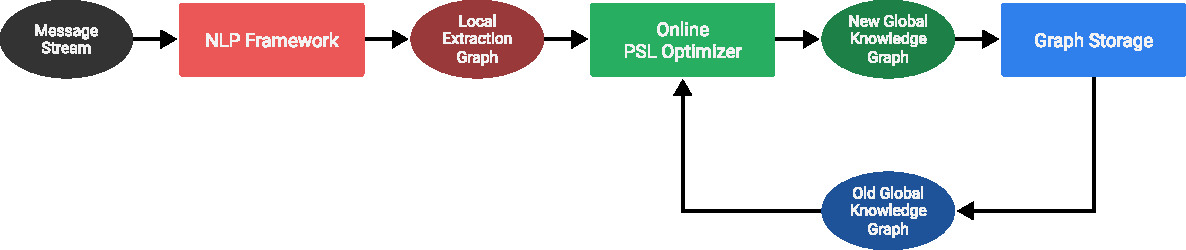
\includegraphics[width=\linewidth]{assets/overview}
	\caption{Vorläufiges grobes Strukturdiagramm des Verfahrens}\label{fig:overview}
\end{figure}

\subsection{Inhaltsverzeichnis}

\begin{enumerate}
	\item Einleitung
		\begin{itemize}
			\item Hintergrund
			\item Problemstellung
			\item Ziele
		\end{itemize}
	\item Literaturüberblick
		\begin{itemize}
			\item Generelle Konstruktionsansätze für Wissensbasen
			\item Information Extraction im Kontext des Natural Language Processings
			\item Ansätze zur automatisierten Wissensgraphkonstruktion
		\end{itemize}
	\item Theoretische Grundlagen
		\begin{itemize}
			\item Open Information Extraction
			\item Markov Random Fields
			\item Modellierung von Hinge-Loss-MRFs mit PSL
			\item Online Optimierung von HL-MRFs mit BOCI
		\end{itemize}
	\item Vorgeschlagenes Wissensgraphkonstruktionsverfahren
		\begin{itemize}
			\item Grundidee
			\item Graph-Persistenzschicht
			\item NLP-Phase
			\item Graphkonstruktionsphase
		\end{itemize}
	\item Ergebnisanalyse
		\begin{itemize}
			\item Testmethode
			\item Ergebnisse
			\item Zusammenfassung und Ausblick
		\end{itemize}
\end{enumerate}

\subsection{Zeitplan}

\begin{figure}[h]
	\centering
	\begin{ganttchart}[
		x unit = 0.9cm,
		y unit title = 0.6cm,
		vgrid,
		canvas/.style = {
			draw = none
		},
		title label font = \sffamily,
		title height = 1,
		title/.style = {
			draw = none,
			fill = none
		},
		bar label font = \sffamily,
		bar label node/.append style = {
			left = 0.2cm
		},
		bar/.append style = {
			fill = blau,
			draw = none
		}
	]{1}{12}
		\gantttitle{Woche}{12} \\
		\gantttitlelist{1,...,12}{1} \\ % ignore triple dots: chktex 11

		\ganttbar{Literaturrecherche}{1}{2} \\
		\ganttbar{Prototyp}{2}{2} \\
		\ganttbar{Implementation}{3}{6} \\
		\ganttbar{Auswertung}{7}{8} \\
		\ganttbar{Schreiben}{6}{11} \\
		\ganttbar{Präsentation}{11}{12}
	\end{ganttchart}
	\caption{Vorläufiger Zeitplan}\label{fig:timeSchedule}
\end{figure}

\bibliographystyle{unsrtnat}
\bibliography{proposal}

\end{document}
